\section{Saturday 0602}


\subsection{Information Extraction 1}
Empire A

\subsubsection{\cite{Gupta2018Joint} Joint bootstrapping machines for high confidence relation extraction}
\begin{itemize}
	\item Challenge: semantic drift
	\item solution: BREX. Use entity and template seeds jointly
\end{itemize}

\subsubsection{\cite{Wang2018Label-Aware} Label-aware double transfer learning for cross-specialty medical NER}
\begin{itemize}
	\item Problem: NER from electronic medical records
	\item Framework: See figure
	\item Optimization goal: $\mathcal{L_{crf}} + \alpha \mathcal{L}_{La-MMD} + \beta \mathcal{L_p} + \gamma \mathcal{L}_{\text{regularizer}}$, CRF + La-MMD loss + parameter similarity loss + regularization.
\end{itemize}
\begin{figure}[h]
	\centering
	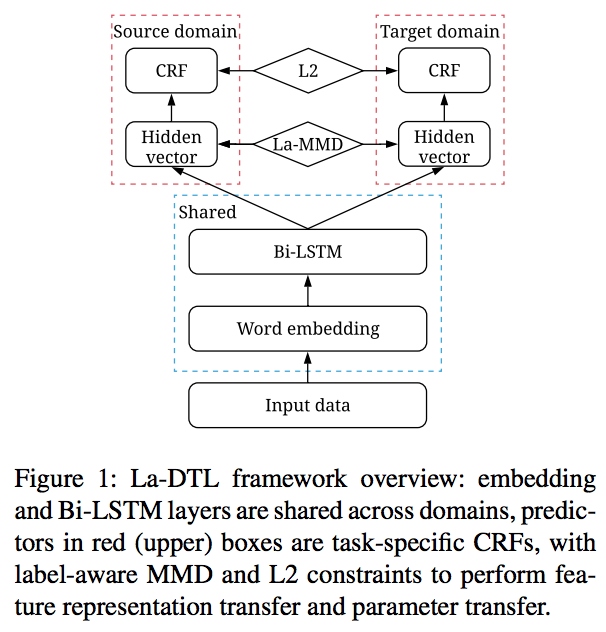
\includegraphics[scale=0.9]{fig0602/LA-MMD}
\end{figure}

\subsection{Morning Poster:  Discourse and Pragmatics 1}
Elite Hall A

\subsubsection{\cite{Schulz2018Multi-Task} Multi-task learning for argumentation mining in low-resource settings}
\begin{itemize}
	\item Task: argumentation mining: segment a text into argumentative and non-argumentative components and identify them. 
	\item: Method: MTL (training a system to solve several conceptually different AM tasks jointly) improves performance over learning in isolation.
\end{itemize}

\subsubsection{\cite{Fu2018Natural} Natural answer generation from heterogeneous memory}
\begin{itemize}
	\item Task: Seq2seq sentence-in sentence-out QA
	\item Problem: Information come from heterogeneous information sources.
	\item Proposed model: Incorporate three components in the decoder hidden state: $h_n$, predicting words from the vocabulary, $h_k$: key pointer, $h_v$, value pointer. Use a gate to mix them, so the resultant network is optimizable through back propagation.
\end{itemize}


\subsubsection{\cite{Baly2018Integrating} Integrating stance detection and fact checking in a unified corpus}
\begin{itemize}
	\item Problem: (part of) fact checking. Decide whether a claim is relevant to a document, and decide whether the document supports the claim.
	\item This work describes the corpus and evaluated using some algorithms someone used in competition. Also referring to their another work next Monday: \cite{Mohtarami2018Automatic}
\end{itemize}

\subsubsection{\cite{Novikova2018RankME:} RankME: reliable human ratings for natural language generation}
\begin{itemize}
	\item Problem of human rating for NLG: consistency, distinct criteria, relative assessment, etc.
	\item Solution: rank-based Magnitude Estimation (RankME), with relative ranking on continuous scale.
	\item How to assess the rating? Intra-class correlation coefficient (ICC)
\end{itemize}


\subsubsection{\cite{Mitcheltree2018Using} Using aspect extraction approaches to generate review summaries and user profiles (Airbnb)}
\begin{itemize}
	\item Task: Aspect extraction. Subtasks: (1) extract a representative sentence from a set of listing-specific reviews for a number of pre-defined aspects (e.g: cleanliness, location). (2) The suitability of aspect embeddings to represet guest profiles.
	\item Comparison between KMeans and ABAE (Attention-based aspect extraction. He et al., 2017), both of which are much better than LDA in these aspect extraction tasks.
\end{itemize}


\subsection{Machine Learning 1}
Empire A

\subsubsection{\cite{Rei2018Zero-Shot} Zero-shot sequence labeling: transferring knowledge from sentences to tokens}
\begin{itemize}
	\item Task: give each token in a sentence a label (of what?), without telling the model how to predict
	\item Previous work to visualize LSTMs using e.g., attention weights, usually work on only a few data samples, and qualitatively.
	\item Method: First train a word LSTM (with attentions) on the classification task (e.g. the uncertainty prediction task), and that attentions show which tokens are the most important. This is the golden annotation $y$. Also the supervised learning "upper bound" baseline.
	\item Where does the zero-shot learning come from? Given this trained network, perform a "backprop from pseudo-label" operation, assuming the pseudo-label is 0. Calculate the gradients at the words. For those whose labels are already 0, the gradients shall be small. Those words labeled as 1 should have large gradients. In this paper, this threshold is set to 1.5 deviation.
\end{itemize}
\takeaway{ The evaluation should be those of the supervised classifier's accuracies -- zero-shot learning can \emph{not} give this kind of per word accuracies. But visualizing the magnitude of gradients is a good idea to visualize LSTMs.}




\subsection{Machine Learning 2}
Empire A
\subsubsection{\cite{Benton2018Deep} Deep dirichlet multinomial regression}
\begin{itemize}
	\item Topic models. e.g. supervised topic models. What if the etadata are high-dimensional, structured, or may not directly relevant to modeling topics.
	\item Backbone: LDA. Change to DMR: sample from document-specific priors. 
	\item From DMR to deep DMR
	\item Trained with Gibbs sampling.
\end{itemize}

\subsubsection{\cite{Rooshenas2018Training} Training structured prediction energy networks with indirect supervision}
\begin{itemize}
	\item Structured prediction
	\item Parameterize energy function over y as a DNN -> can find the min of E using gradient descent.
	\item Supervised learning: Structured SVM (Belanger and McCallum, 2016)
	\item Indirect supervision 
	\item Rank-based training
\end{itemize}


\subsubsection{\cite{gallagher2016anchored} Anchored correlation explanation: topic modeling with minimal Domain Knowledge}

\begin{itemize}
	\item How to do topic modeling with thousands of information bottleneck?
	\item LDA is a a generative topic model. Goods and bads of generative modelings.
	\item Topic model that learns topics through information-theoretic criteria.
	\item CorEx (total Correlation Explanation): a topic is a binary latent factor. Goal: find factors that make words conditionally independent. 
	$$ \min_Y TC(W_1 .. W_n | Y) = \min_Y D_{KL} \left ( p(w_1, .. w_n | y) || \Pi_i p(w_y | y) \right )$$
	$TC(W|Y)=0$ iff the topics "explain" all the dependence (total correlation). Here comes the Correlation Explanation name.
	\item Then rewrite the objective as mutual information
	$$\min_Y \Sigma_i I(Y_j : W) - \Sigma_i \alpha_{i,j} I(W_i; Y_j)$$
	where $\alpha_{i,j} = \frac{I(W_i : W_j | Y_{k \neq j})}{I(W_i : Y_j)}$, which is the unique information in $Y_j$ about $W_i$
	
	Then transform a combinatorial to a continuous optimization

	\item Extensions: (1) hierarchical CorEx; (2) semi-supervised learning.
	\item Anchored CorEx objective is exactly maximizing the information bottleneck.
\end{itemize}


\subsubsection{\cite{zhang2017aspect} Aspect-augmented adversarial networks for domain adaptation }

\begin{itemize}
	\item Problem: Transfer learning, but both source and target classifiers operate over the same domain.
	\item Method: Learn a document-level representation that is hard to tell the domain, but easy to tell the class label.
	\item The encoder contains:
	A CNN per sentence; Improve adversarial training by reconstruction.
	\item Apply relevance score using a small set of keyword rules. 
\end{itemize}
\begin{figure}[h]
	\centering
	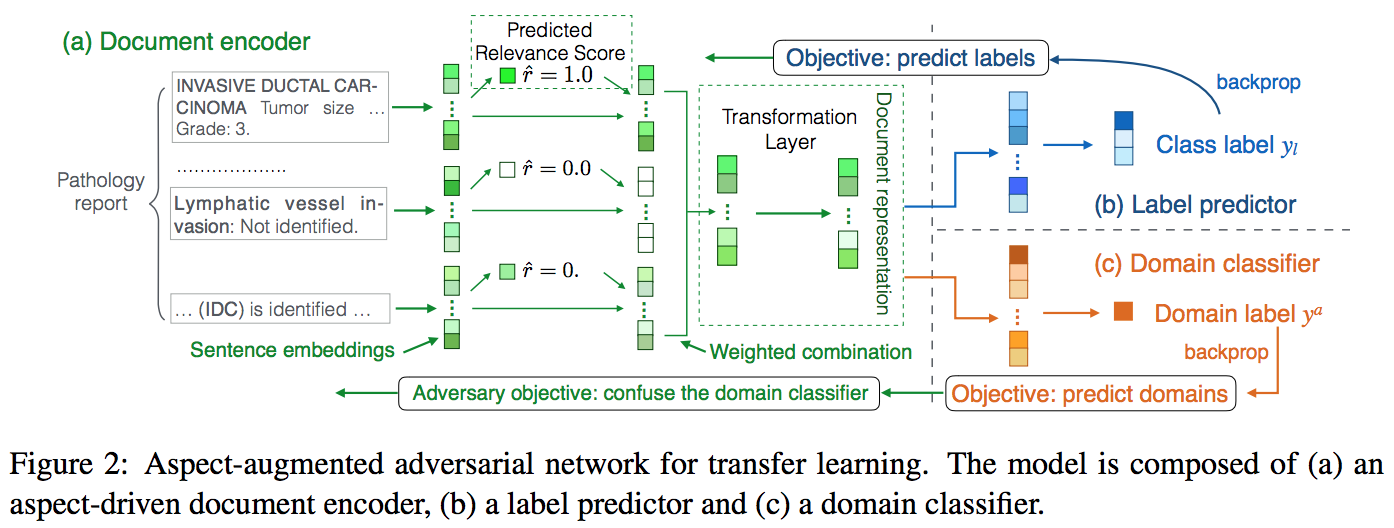
\includegraphics[scale=0.6]{fig0602/zhang2017aspect}
\end{figure}


\subsection{SRW highlights}
Empire C

\subsubsection{\cite{Ezeani2018Igbo} Igbo diactritic restoration using embedding models}
\begin{itemize}
	\item Igbo language: more spoken than written, and low-resource for NLP. (mostly south-eastern Nigeria)
	\item Problem: diacritic ambiguity (same wordkey, but different meanings)
	\item Embedding projection: align English embedding to Igbo language, using an alignment dictionary.
	\item Diacritic retoration proces: during evaluating candidate instances, choose the one with the maximum (cosine?) similarity in the embedded vector.
\end{itemize}

\subsubsection{\cite{Acharya2018Towards} Towards generating personalized hospitalization summaries}
\begin{itemize}
	\item Problem: summarization
	\item Method: FIrst build concept graph via UMLs, extract physician / nursing concepts to include. Then simplify. Then Arrange event ordering.
\end{itemize}

\subsubsection{\cite{Shin2018Alignment} Alignment, acceptance, and rejection of group identities in online political discourse}
\begin{itemize}
	\item Trump and Clinton supporters tend to use and align pronouns differently.
	\item Their rhetorical words are not substantially different.
\end{itemize}